\begin{figure}[H]
\caption{Microservice Architecture Style Structure}
\centering
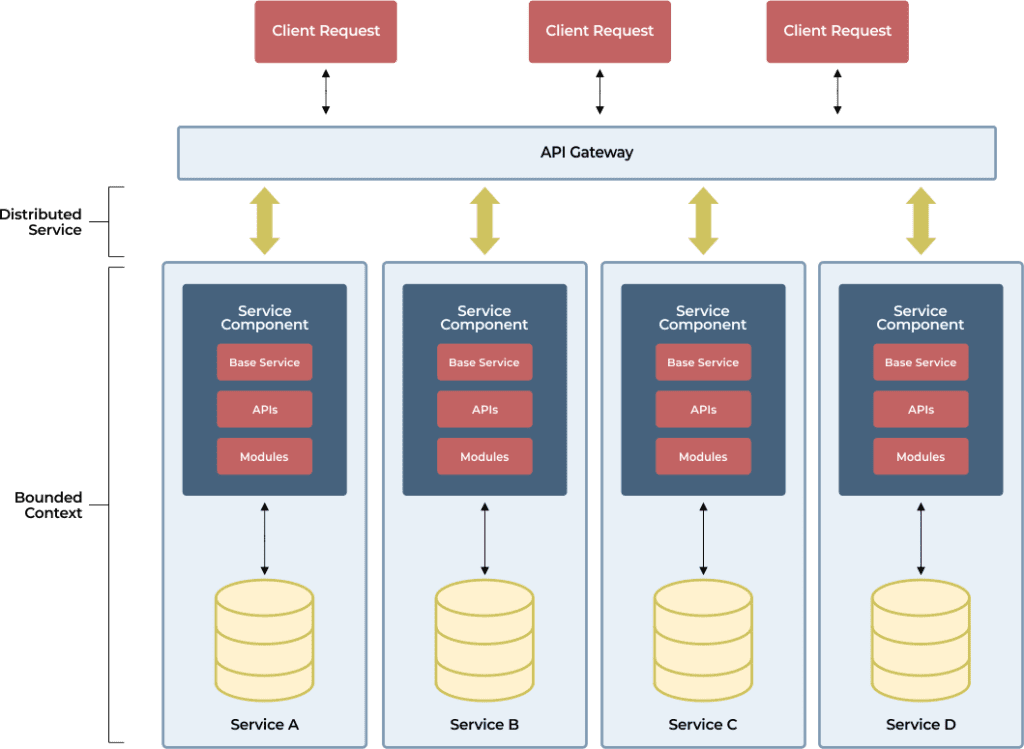
\includegraphics[width=1\linewidth]{images/Microservice-Architecture-img-1-1024x749.png}
\small
\textit{Note.} The image depicts a microservices architecture diagram. At the top of the diagram, there are three \textbf{"Client Request"} boxes, representing incoming requests from clients. Below the client requests is an \textbf{"API Gateway"} layer, which serves as the entry point for all client requests. The main body of the diagram shows \textbf{four separate services} (Service A, B, C, and D), representing a distributed service architecture.
\textit{Creator.} (\cite{micro})\footnote[40]{\fullcite{micro}}
\end{figure}